%!TEX root = labo.tex
\setcounter{chapter}{3}
\chapter{Wireless Security}

In this lab, you will have a look at the impact of various security measures which are available for wireless networks. The main goal is to show what the effect is of a certain security method and what a possible attacker/sniffer can do on the protected network. In the first lab, you already performed some sniffing using the monitor mode. It should be clear that unless we take some security measures, it is quite easy to intercept and read any management information and data from open networks. It is even quite easy to perform \ac{dos} attacks on open networks as you will see at the end of this lab.

In the first part of the lab, you will investigate the more basic security features like hiding a network and \ac{mac} filtering. In the second part, you will have a look at encryption mechanisms and try to hack some of these. In the last part, we will introduce some basic attacks. These attacks are introduced to illustrate the mechanisms behind wireless networks and should only be used for this purpose.

\section{Basic Security Measures}


\begin{figure}[h!]
	\begin{center}
		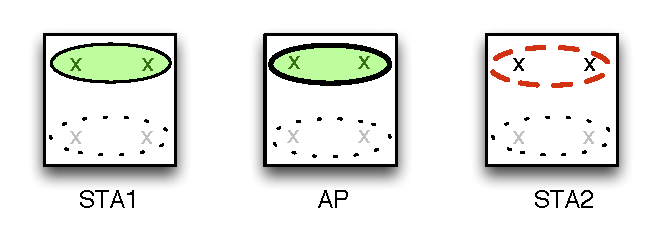
\includegraphics[width=0.5\textwidth]{images/macfilter.pdf}
		\caption{MAC filter setup} 
		\label{fig:macfilter} 
	\end{center}
\end{figure}

\begin{exercise}{Network hiding}

A first step in preventing someone to use your wireless network is to hide it from being detected by a regular scan. Hiding a \ac{ssid} ensures it will not show up in the list of available \acp{ap} when a scan is performed. You will however show that the clever sniffer is still able to detect the network.

\begin{enumerate}
	\item Set up your network as illustrated in figure \ref{fig:macfilter}, but do not set up the \ac{wnic} of \ac{sta}1 yet. \label{ex:ssidHiding1}
	\item Start a trace on the monitor interface (\file{\acs{sta}2.pcap}) of \ac{sta}2. While the trace is running, bring up the \ac{wnic} from \ac{sta}1. \label{ex:ssidHiding2} Make sure the station is associated with the \ac{ap} before you stop your trace.
	\item Indicate in which frames the \ac{ssid} is visible. Give a packet ID of an example packet in your trace file for each.\newline
	\begin{esolution}
	\end{esolution} 
	\item The next step is to hide the \ac{ssid}. This can be done adding the following line to the hostapd.conf file: \incommand{ignore\_broadcast\_ssid=1}. Bring the interface down on \ac{sta}1, restart \incommand{hostapd} on the \ac{ap} and repeat steps \ref{ex:ssidHiding1} and \ref{ex:ssidHiding2}. Save your trace to \file{STA2.pcap}.
	\item Compare the two trace files and indicate how the \ac{ssid} is hidden. In what way can a \ac{ssid} still be detected?\newline
	\begin{esolution}
	\end{esolution}
\end{enumerate}

\end{exercise}

\begin{exercise}{\ac{mac} filtering}

Continuing from the setup you used in the previous exercise, a possible intruder has still complete access to our network. In the next step, you will prevent him from joining the network by \ac{mac} filtering. 


\begin{enumerate}
	\item The management of the \ac{mac} filtering is also performed by modifying the \incommand{hostapd.conf} file at the \ac{ap}.  The entries needed for \ac{mac} filtering are:
	\begin{description}
		\item[macaddr\_acl=] controls the behaviour of the mac filtering  and expects an integer value from the following list:
		\begin{description}
			\item[0] accept unless in deny list,
			\item[1] deny unless in accept list,
			\item[2] use external RADIUS server (accept/deny lists are searched first
		\end{description}
		\item[accept\_mac\_file=] append the name of the file here that contains the list of \ac{mac} addresses to accept.
		\item[deny\_mac\_file=] append the name of the file here that contains the list of \ac{mac} addresses to deny.
	\end{description} 
	\item Configure the \ac{ap} in such a way that the \ac{mac} address of the \texttt{wlan0} interface of \ac{sta}1 is blocked from the network. SSID broadcasting may be enabled again.
	\item Now bring down the \ac{wnic} at \ac{sta}1 again, restart a capture session on \ac{sta}2 and save it to \file{\acs{sta}2.pcap}\\ and bring the \ac{wnic} back up at \ac{sta}1 when this capture session is active. Compare the results from this capture file with the first one you made and discuss the differences between both. Illustrate with packet IDs.\newline
	\begin{esolution}
	\end{esolution}
	\item Of course, in a real world setup, blocking unwanted MAC addresses is not feasible. One would use the option with the \texttt{accept\_mac\_file} parameter, allowing only known \ac{mac} addresses to connect. How would you circumvent this security measure? If an attacker has joined the network, will this have an effect on legitimate stations on that network?\newline
	\begin{esolution}
	\end{esolution}
\end{enumerate}

	
\end{exercise}




\section{Encryption}
\subsection{\acs{wep}}

The security techniques from the previous section will ``prevent'' a possible attacker from joining the network by hiding the network or preventing him access to the network. However, it is still possible to read any communication over the network by using a \ac{wnic} in monitor mode. Encryption mechanisms will counter this and obfuscate the network traffic for an eavesdropper. You will take a look at \ac{wep} here as this method is still sometimes being used although it is very vulnerable to attacks. \ac{wpa}2 is far more resilient.

\begin{exercise}{\ac{wep} encryption}
\label{ex:wep}

	\ac{wep} was the first available encryption method, standardised together with the \wifi standard. It was however quickly been proven insecure. In fact, as of 2004, \ac{wep} was declared deprecated by IEEE because of its flaws. In this exercise, you will first set up a \ac{wep} encrypted network to check what is exactly encrypted. In the next exercise you will crack the encryption key.
	
Because \ac{wep} is quite old, the tools you will use assume that IPv4 is used, as they will use \ac{arp} messages. Therefore, for this exercise, you will configure IPv4 addresses instead of IPv6 addresses.

\begin{figure}[h!]
		\begin{center}
			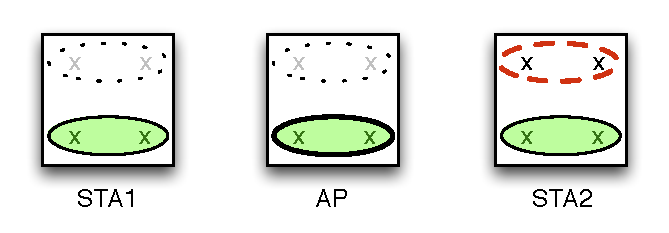
\includegraphics[width=0.5\textwidth]{images/wepcrack.pdf}
			\caption{WEP setup} 
			\label{fig:wepcrack} 
		\end{center}
	\end{figure}
	
	\begin{enumerate}
		\item Start from the network setup as shown in figure \ref{fig:wepcrack}. Disable any \ac{mac} filter that is still in place.
		\item In order to avoid capturing needless IPv4 traffic, disable the \texttt{avahi-daemon} on all three nodes:\newline
		\command{\prompt{\acs{wmn}} killall avahi-daemon}
		\item Create a tracefile on the monitor interface of \ac{sta}2 (\file{\ac{sta}2.cap}\\), containing the scan, authentication and association phase of \ac{sta}1 and a 5 packet ping session between \ac{sta}1 and \ac{sta}2. Use \texttt{10.0.\acs{gid}.1/24} for \ac{sta}1 and \texttt{10.0.\acs{gid}.2/24} for \ac{sta}2.\newline
		\command{\prompt{\acs{sta}} ip addr add 10.0.\acs{gid}.X/24 broadcast 10.0.\acs{gid}.255 dev wlan1}
		\item Make sure that \ac{sta}2 is connected to the \ac{ap} and that the \ac{wnic} of \ac{sta}1 is down before the start of the capture session. To ping, use \incommand{ping} instead of \incommand{ping6}. This trace will be our reference trace. \label{wep1} 
		\item Activate the \ac{wep} encryption on the \ac{ap}. You can choose a random key as long as it is either 5 or 13 characters long ("arandomwepkey" in this example):\newline
		Change the \incommand{hostapd.conf} file, so that it includes the following lines:\newline
		\command{wep\_key0="arandomwepkey"}
		\command{wep\_default\_key=0}
		\remark The WEP key must be \stress{exactly 5 or 13} characters long!
		\item Make sure the \ac{ap} is running. Connect \ac{sta}2 to the \ac{ap}:\newline
		\command{\prompt{\acs{sta}2} iw dev wlan1 connect wmn-0-A key 0:arandomwepkey}
		\item Make sure the interface of \ac{sta}1 is down and then start a new trace on the monitor interface of \ac{sta}2. Save it to \file{\acs{sta}2.wep.pcap}\\.
		\item Perform the same test as in step \ref{wep1}, but be sure to add \texttt{key 0:arandomwepkey} when you connect \ac{sta}1 to the network.
		\item Compare both trace files. In the second trace file, you should no longer be able to see the \incommand{ping} session in the clear.
		\begin{itemize}
			\item Which frame types are encrypted?\newline
			\begin{esolution}
			\end{esolution}
			\item Which part of a frame is encrypted and which part is still readable?\newline
			\begin{esolution}
			\end{esolution}
		\end{itemize} 
		Refer to specific frames from the second trace file to illustrate your answers.
		
	\end{enumerate}
	
\end{exercise}
	
	
	
\begin{exercise}{Cracking the \ac{wep} keys}	

	Without going into details about the flaws in  \ac{wep}, the main problem arises from the fact that traffic keys are easily repeated on a busy network. A traffic key is the key actually used by the encryption algorithm RC4.  As RC4 is a stream cipher, the same key should not be used twice. Therefore, the shared \ac{wep} key, which is configured in each \ac{ap} and \ac{sta}, is combined with a random \ac{iv}. This \ac{iv} is transmitted in plaintext between two wireless clients so the receiver can recreate the encryption key used for a specific packet, by combining the chosen (shared) network key with the received \ac{iv}. As the \ac{iv} has a length of only 3 bytes, the number of possibilities is relatively low and in busy networks, the same \acp{iv} are frequently reused, weakening the cryptographic strength of \ac{wep}. Furthermore, statistical relations between used keys and encrypted text can be exploited to find the used key.
	
	Various methods have been developed to crack a \ac{wep} key, but you will just illustrate the mere ease with which a \ac{wep} encrypted network can be hacked using the aircrack tool \cite{aircrackNG}. This tool implements various approaches, but you will limit ourselves to \ac{ptw} method. The attack is based on the fact that the first 16 bytes of an \ac{arp} packet are fixed. This is also the reason we switched to IPv4 for this exercise\ldots For more details read \cite{cryptoeprint:2007:120}, specifically sections 1 and 5 for a general overview. Exploiting the relation between cleartext and the captured \acp{iv} makes it possible to quite easily determine the network key.
	
	\begin{figure}[h!]
		\begin{center}
			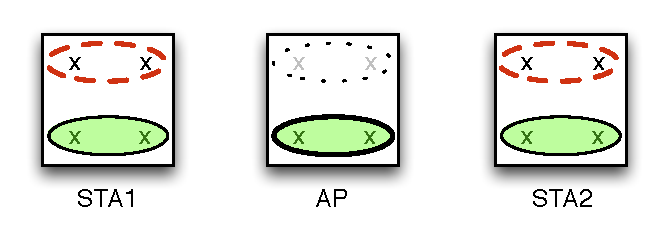
\includegraphics[width=0.5\textwidth]{images/wepcrack2.pdf}
			\caption{WEP cracking setup} 
			\label{fig:wepcrack2} 
		\end{center}
	\end{figure}
	
	
	\begin{enumerate}
		\item Before you start to crack the configured \ac{wep} key, first have a second look at the traces from the previous exercise. Using Wireshark\cite{wireshark}, you can decrypt an encrypted trace. Using the menu Edit$\rightarrow$ Preferences $\rightarrow$ Protocols $\rightarrow$ IEEE 802.11 you can specify the key in HEX. To convert your key to HEX, use e.g. the following website: \url{http://www.dirtymonday.net/key_convert.html} For our example it will be \incommand{6172616E646F6D7765706B6579}.\newline
Make sure you also check the `decrypt packets' box. Select an ICMP request in both trace files (unencrypted and encrypted, but decrypted by Wireshark) and identify the extra information added to a frame in order to encrypt it. Also indicate where in the frame this information is added.\newline
		\begin{esolution}
		\end{esolution}
		\item Start from the \ac{wep} encrypted network you created in the previous exercise.
		\item Add an additional monitor interface on \ac{sta}1, resulting in the network scheme shown in figure \ref{fig:wepcrack2}. The monitor interface on \ac{sta}2 will be used to perform the actual attack. \ac{arp} packets will be injected into the network in order to trigger \ac{arp} responses which will contain new \acp{iv} with every response . These packets will be captured and stored in files. In parallel with this capturing of new \ac{arp} responses and the associated \acp{iv}, we can start the process of analyzing these packages and searching for the key. The monitor interface on \ac{sta}1 will be used to monitor the channel so we can afterwards take a look at what happened.
		\item Start a packet capture to \file{\acs{sta}1.pcap}\\ on the monitor interface of \ac{sta}1.
		\item Start the \ac{iv} capture process at \ac{sta}2. This command will store its captured frames in files \incommand{output-xy.cap} and \incommand{output-xy.txt}. Make sure to run this command with your active directory set to the \texttt{/mnt} folder, in which a remote directory is mounted.\newline
		\command{\prompt{STA2} airodump-ng --band a --channel x --bssid <\acs{mac} addr \acs{ap}> -w output wlan0}
		This should give you an overview screen where at least the incoming beacon count is rising. If no activity is shown, bring the interface down and then bring it up again and retry. This command will store its captured frames in files \incommand{output-xy.cap} and \incommand{output-xy.txt}. Make sure to run this command in \texttt{/mnt}, where a remote location is mounted.\newline
		\item On a new terminal, perform a fake authentication to the \ac{ap} from the attacking machine (\ac{sta}2). This ensures the frames we will be injecting for \texttt{wlan1} will be accepted by the \ac{ap}:\newline
		\command{\prompt{STA2} aireplay-ng --fakeauth 0 -e wmn-\acs{gid}-A -a <\acs{mac} addr \acs{ap}> -h <\acs{mac} addr wlan0> wlan0.}	
		\item It is now time to actively inject packets into the wireless network. This is done by the following command:
		 \command{\prompt{STA2} aireplay-ng --arpreplay -b <MAC addr AP> -h <MAC addr wlan0> -x 1024 -o 512 wlan0}\newline
		 This command will monitor incoming packets and when an \ac{arp} request passes, it will re-inject it at a rate of several 100 frames/s.  You should be able to see this in the output from \incommand{airodump-ng}.\newline
		 \remark Due to a bug in the driver, the packet injection rate will not be high enough. You should run 10 of the above \incommand{aireplay-ng} commands in parallel to generate enough packets. You can do so easily by editing the \texttt{wepcrack.sh} script found on the nodes. Insert the correct \ac{mac} addresses in that script and run it. To stop the replay attack, simply type \incommand{killall aireplay-ng}.
		  \item In order to get an \ac{arp} request, just start a ping from \ac{sta}1 to \ac{ap}. This should trigger an \ac{arp} request. If the \ac{arp} tables already contained the IP addresses from both hosts (check it with \incommand{\prompt{STA1} ip neigh}), remove the entry using \incommand{ip neigh flush dev wlan1}.
		 \item To crack the key, the tool \incommand{aircrack-ng} can be used. This tool processes the files generated by \incommand{airodump-ng}. The needed number of packets to crack the key depends on the bit length of the key. In general, you need at least 20,000 packets for a 64-bit key and between 40,000 and 85,000 for a 128-bit key. To start the analysis, run the following command in the folder containing the output from \incommand{airodump-ng}:\newline
		\command{\prompt{STA2} aircrack-ng -b  <\acs{mac} addr \acs{ap}> output*.cap -q}
		\item If you captured enough packets, after a while, the \incommand{aircrack-ng} tool should provide you with the \ac{wep} key used in your network. Copy its output here:\newline
		\begin{esolution}
		\end{esolution}
		\item Using the following \incommand{tshark} command on a lab PC, you can get a list of \acp{iv} used during your session. \newline
		\command{tshark -r <trace file> -T fields -e wlan.wep.iv}
		\item How many \acp{iv} did you capture? And how many of them occured at least twice?\newline
		\begin{esolution}
		\end{esolution}	
	\item When handing in the report, you must include the \texttt{output-*.csv} and \texttt{*.netxml} files. \texttt{output-*.cap} is not required, as it will be quite large. Limit the trace file of \ac{sta}1 to only a few (e.g. a hundred) of packets that show the \ac{arp} injection in progress.
	\end{enumerate} 
		
\end{exercise}

\subsection{\acs{wpa}2}

As you have demonstrated in the previous exercise, \ac{wep} encryption is easily circumvented. You will now take a look at \ac{wpa}2 encryption. You will no try to crack it, as \ac{wpa}2 uses the \ac{ccmp} algorithm with \ac{aes} encryption, which is extremely resilient to attacks. To give you an idea, the best known method until now to crack a 128 bit \ac{aes} key, which is used by \ac{wpa}2, still takes at least \( 2^{126.1} \) computations\cite{cryptoeprint:2011:449}.

A security flaw concerning \ac{wps} has been discovered that makes \acp{ap} running \ac{wps} vulnerable to a relatively easy attack (which would still take far too much time for this lab exercise)\cite{wps}. This, of course, does not hold true for \acp{ap} that do not have \ac{wps} enabled. If you want to read up on how \ac{wpa}2 works and on the evolution in security from \ac{wep} over \ac{wpa} to \ac{wpa}2, you should read \cite{wifisecurity:2012}.

\begin{exercise}{\acs{wpa}2}

\begin{figure}[h!]
		\begin{center}
			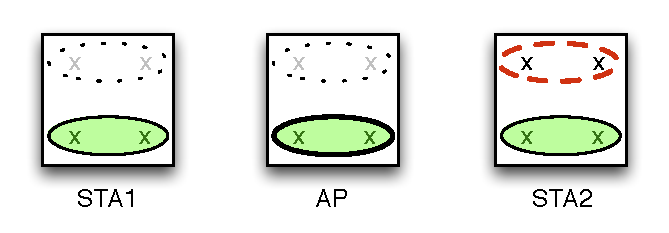
\includegraphics[width=0.5\textwidth]{images/wepcrack.pdf}
			\caption{\acs{wpa} setup} 
			\label{fig:wpa} 
		\end{center}
	\end{figure}

\begin{enumerate}
	\item Start from the \ac{wpa}2 enabled network setup as seen in figure \ref{fig:wpa}.
	\item On the \ac{ap}, to enable \ac{wpa}2, make sure that the line \texttt{wpa=0} in the \texttt{hostapd.conf} file is changed to \texttt{wpa=2}, and add the following lines to \texttt{hostapd.conf}:
	\begin{verbatim}
		wpa_passphrase=aRandomPassphrase
		wpa_key_mgmt=WPA-PSK
		rsn_pairwise=CCMP
	\end{verbatim}
	\remark Use your own passphrase if you like. Unlike \ac{wep}, it is not restricted to a certain amount of characters.
	\item Set the IP addresses of \texttt{wlan1} on \ac{sta}1 and \ac{sta}2 to \texttt{fc00:\acs{gid}::1/64} and \texttt{fc00:\acs{gid}::2/64}, respectively.
	\item Connect \ac{sta}2 to the network. In order to do so, modify the \texttt{wpa\_supplicant.conf} file so that it includes the correct \acs{essid} and passhprase. Afterwards, run:\newline
	\command{\prompt{\acs{sta}2} wpa\_supplicant -B -c/root/wpa\_supplicant.conf -iwlan1}
	\remark You might get an error like \texttt{ioctl[SIOCSIWENCODEEXT]: Invalid argument}. You can safely ignore this error.
	\item Make sure the monitor interface on \ac{sta}2 is configured and start a trace. Save it in \file{\acs{sta}2.pcap}\\.
	\item Now bring the interface on \ac{sta}1 up an do \texttt{ping6 -c 5} to \ac{sta}2.
	\item Which frame types are encrypted? Give examples.\newline
		\begin{esolution}
		\end{esolution}
	\item Which part of a frame is encrypted and which part is still readable?\newline
		\begin{esolution}
		\end{esolution}
		\item Compare this trace file with the one made in exercise \ref{ex:wep}. Compare the authentication/association phase of \ac{sta}1. What are the similarities and what are the differences? Refer to packet IDs!\newline
		\begin{esolution}
		\end{esolution}
		\item Now, compare an encrypted frame in both traces. Indicate where they differ.\newline
		\begin{esolution}
		\end{esolution}
\end{enumerate}

\end{exercise}



\section{Denial of Service Attacks}

\begin{figure}[h!]
		\begin{center}
			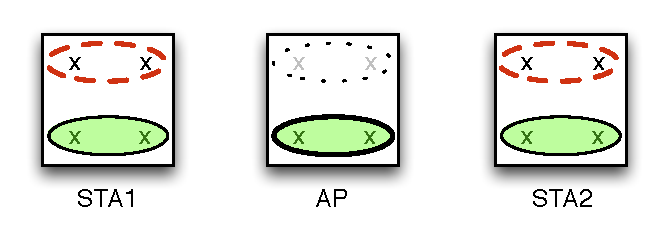
\includegraphics[width=0.5\textwidth]{images/wepcrack2.pdf}
			\caption{DoS setup} 
			\label{fig:dos} 
		\end{center}
	\end{figure}

In the previous section, you have gained access to a \ac{wep} encrypted network by actively injecting packets and cracking the key. This kind of attack makes it possible that you, the attacker, can afterwards associate with the network and sniff all traffic on that network. Alternatively, you can also use the network yourself as if you were a normal user.

Within this section, you will illustrate a \ac{dos} attack that shows the vulnerability of a wireless network. You will not gain access to the network as such, but you will disturb normal network operation. Tools to do so are freely available and current encryption techniques cannot prevent these attacks as they make use of management frame injection. As you have seen, management frames are not encrypted and thus can be easily injected into a wireless network. 

\begin{exercise}{Disassociation Attack}
	
	The principle behind a disassociation attack is quite easy. A disassociation frame is sent by either a \ac{sta} or \ac{ap} to signal the disconnection from the wireless network. For instance, it is sent by a \ac{sta} just before you disable an associated \ac{wnic}. Although the sending of a disassociation message is not mandatory by the standard, at reception of such frame, a client should consider its connection lost and an \ac{ap} will remove a \ac{sta} from the list of connected stations. Injecting a malicious disassociation frame for a wireless node will thus force this node to scan for and associate again to its \ac{ap}, resulting in a connectionless period. If the disassociation frame is sent periodically, this can render the wireless network useless to the attacked \ac{sta}.

\begin{enumerate}
	\item Start from the network scheme as illustrated in figure \ref{fig:dos}.
	\item Be sure to have configured your network with \ac{wpa}2 encryption.
	\item Configure the IP addresses of \ac{sta}1 and \ac{sta}2  to \texttt{fc00:\acs{gid}::1/64} and\newline \texttt{fc00:\acs{gid}::2/64} respectively.
	\item On the monitor interface of \ac{sta}1, start a capture session and save it to\newline \file{\acs{sta}1.pcap}\\.
	\item Start a \incommand{ping6} from \ac{sta}1 to \ac{sta}2.
	\item On \ac{sta}2, use the following command to send a disassociation to \ac{sta}1:\newline
	\command{\prompt{STA2}  aireplay-ng --deauth 1 wlan0 -a <MAC addr AP> -c <MAC addr STA1>}
	\item What is the result for the ping?\newline
	\begin{esolution}
	\end{esolution}
	\item Open the trace file and explain using this trace what exactly happened.\newline
	\begin{esolution}
	\end{esolution}

\end{enumerate} 	
	
\end{exercise}
